
\documentclass[12pt]{article}

\usepackage{graphicx}
%\usepackage{subcaption}
\usepackage{amsmath}
\usepackage{amssymb}
%\usepackage{afterpage}
%\usepackage{showlabels}
% \usepackage{epstopdf}
% \usepackage{pdfpages}
\usepackage{geometry}
%\usepackage{wrapfig}
\usepackage{url}
\usepackage{times}
\usepackage{pdfpages}
\usepackage{etoolbox}
\usepackage{hyperref}
\usepackage{enumitem}
\hypersetup{
    colorlinks=true,
    linkcolor=blue,
    filecolor=magenta,
    urlcolor=cyan,
    pdftitle={Overleaf Example},
    pdfpagemode=FullScreen,
    }

\urlstyle{same}

\newcommand{\s}{\textrm{s}}
\newcommand{\m}{\textrm{m}}
\newcommand{\kg}{\textrm{kg}}
\newcommand{\N}{\textrm{N}}
\DeclareMathOperator{\sech}{sech}
\DeclareMathOperator{\arctanh}{arctanh}

\newcommand{\shortlist}{%
\parindent 0in%
\parskip   0in%
\itemsep   0in%
\topsep    0in%
\parsep    0in%
}

\setlength{\parindent}{0in}

\geometry{letterpaper,tmargin=1in,bmargin=1in,lmargin=1in,rmargin=1in}

\newcommand{\soln}[2] {\textit{Solution:} #2}

%\renewcommand{\soln}[2] {\vspace*{#1}}

\newcommand{\Title}{PHYS 615 -- HW 6}

\begin{document}

\begin{center}
    {\Large\bfseries\Title}

\end{center}
\bigskip
\bigskip

\textbf{Types of homework questions}
\begin{itemize}\shortlist
    \item	RQ (Reading questions):  prompt you to go back to the text and read and think about the text more carefully and explain in your own words. While not directly tested in quizzes, can help you think more deeply about quiz questions.
    \item	BF (Building foundations):  gives you an opportunity to build and practice foundational skills that you have, presumably, seen before.
    \item	TQQ (typical quiz questions):   Similar questions (though perhaps longer or shorter) will be asked on quizzes.  But the difficulty level and skills tested will be similar.
    \item Design (D):  These are questions in which you are given a desired outcome and asked to figure out how to make it happen.  These will often also be TQQ’s, but always starting with desired motion/behavior as the given.
    \item	COMP (Computing): computing questions often related to TQQ but will never be asked on a quiz (since debugging can take so long).  You will need to do at least four computing questions over the semester
    \item	FC (free choice): allows you to decide where to put your time.  Any of the following are possible:  work through a section of the text or a lecture in detail; redo a problem from before; do an unassigned problem in the text; extend a computing project; try a problem using a different analytical approach (e.g. forces instead of conservation of energy).
    \item ACT (in-class activity): These questions are repeats of questions (or similar to) that occurred in a previous in-class activity.
    \item \textbf{Standard Reading Questions}: How does the reading connect with what you already know? What was something new?  Ask an "I wonder" question OR give an example applying the idea in the reading.
\end{itemize}

\textbf{Please remember to say something about the "Check/Learn" part at the end of solving a problem!}

Full credit will be given at 75\% of the total points possible, so you can choose a subset of problems (you can do more / all, but the score is capped at 75\%)

This homework contains some previous group activities. I'm including them here in order to try to help gradescope, but you can of course hand in the original paper version I handed out in class.

\clearpage

\begin{enumerate}

    \item COMP (15 points) Runge-Kutta integration

          Back quite a while ago, we solved the skateboard in a half pipe problem numerically, and we noticed that even in the linear (small-angle) approximation, the amplitude seemed to grow over time quite substantially unless we used a tiny timestep: \url{https://github.com/germasch/hw/blob/main/notebooks/euler-skateboard.ipynb}

          Our next goal is going to be solving projectile motion with quadratic drag, but before we try to do so (down the road), let's try to get our code to give us a more accurate numerical approximate solution.

          Follow the tutorial at \url{https://lpsa.swarthmore.edu/NumInt/NumIntSecond.html} through "Example 1". As a first step, implement the 2nd order Runge-Kutta method to solve the 1st order ODE $\dot y = -2 y$. (As usual, you can do so in Matlab or Python).

          Once it is working, you can now apply it to the skateboard problem, which we have also written as 1st order ODE previously. Compare the solution we got previously from the Euler method to this hopefully improved method for a timestep of $0.1$ and $0.01$.

          Please hand in your code on Canvas, and include a brief write-up on the results you got (here or on canvas).

          \soln{15em}{See \url{https://github.com/germasch/hw/blob/main/notebooks/rk2.ipynb}}

          \clearpage
    \item TQQ (10 points) Jumping on a merry-go-round [Sorry, this is problem kinda late, I had hoped to have you do this in class at the end of Chapter 3, but well, better late than never...]

          Sarah, with mass $m$ and speed $v$, runs toward a merry-go-round and jumps on at its edge. Sarah and the merry-go-round (mass $M$, radius $R$, and moment of inertial $I = \frac{1}{2}MR^2$) then spin together with angular velocity $\omega_f$. If Sarah's initial velocity is tangent to the circular merry-go-round, what is $\omega_f$?

          \soln{15em}{
              Since this is a (sort of) collision, angular momentum is conserved for the system of merry-go-round and Sarah. The initial angular momentum is Sarah's angular momentum -- who runs in a straight line, but as we've seen in a previous activity, straight line motion does have (constant) angular momentum $mv$ times distance of closest approach, so
              $$L_i = mvR$$
              Afterwards, both Sarah and the merry-go-round are rotating at $\omega_f$:
              $$L_f = \left(\frac{1}{2}MR^2 + mR^2\right)\omega_f$$

              (Note that I used the moment of inertia for a point mass for Sarah -- but I could have also written her angular momentum as $mv_fR = m(R\omega_f)R = mR^2\omega_f$, which gives the same contribution.)

              Setting $L_i = L_f$ and solving for $\omega_f$:
              $$
                  \omega_f = \frac{mvR}{(\frac{1}{2}MR^2 + mR^2)}
              $$
          }

          \clearpage
    \item TQQ (10 points) A particle of mass $m$ is moving on a frictionless horizontal table and is attached to a string, whose other end passes through a hole in the table, where I am holding it. Initially, the particle is moving in a circle of radius $r_0$ with angular velocity $\omega_0$, but I now pull the string down through the hole until a length $r$ remains between the hole and the particle.

          \begin{enumerate}
              \item What's the particle's angular velocity now?

                    \soln{10em}{
                        The net force on the particle is directed along the string toward the center, so it does not exert a torque -- angular momentum is conserved.

                        The angular momentum is initially given by $l_0 = rmv_0 = mr_0^2\omega_0$. At any later time, $r$ and $\omega$ may have changed but angular momentum $mr^2\omega$ is still the same (conserved), so since the mass also doesn't change, $r_0^2\omega_0 = r^2\omega$. So

                        $$\omega = \left(\frac{r_0}{r}\right)^2 \omega_0$$
                    }

              \item Assuming that I pull the string so slowly that we can approximate the particle's path by a circle of slowly changing radius, calculate the work I did pulling the string.

                    \soln{10em}{
                        The tension $F$ in the string must provide centripetal acceleration $v^2/r = \omega^2 r$, so
                        $$F = m\omega^2 r = m\left(\frac{r_0}{r}\right)^4 \omega_0^2 r = m \omega_0^2 r_0^4 \frac{1}{r^3}$$

                        Now I can calculate my work ($dr$ is negative, so the distance the string moves where I'm pulling is $-dr$ and the force is in the same direction):
                        $$W = m \omega_0^2 r_0^4\int_{r_0}^r \frac{-dr'}{r'^3} = \frac{1}{2} m \omega_0^2 r_0^4 \left(\frac{1}{r^2} - \frac{1}{r_0^2}  \right)$$
                    }

              \item Compare your answer to part (b) with the particle's gain in kinetic energy.

                    \soln{10em}{
                        Initially, the particle has kinetic energy
                        $$T_0 = \frac{1}{2}mv_0^2 = \frac{1}{2}mr_0^2\omega_0^2$$
                        Later, it has
                        $$T = \frac{1}{2}mr^2\omega^2 = \frac{1}{2}mr^2 \left(\frac{r_0}{r}\right)^4 \omega_0^2 = \frac{1}{2}m \frac{r_0^4}{r^2} \omega_0^2$$
                        So the change is
                        $$\Delta T = T - T_0 = \frac{1}{2}m \frac{r_0^4}{r^2} \omega_0^2 - \frac{1}{2}m\frac{r_0^4}{r_0^2}\omega_0^2 = \frac{1}{2}mr_0^4\omega_0^2
                            \left(\frac{1}{r^2} - \frac{1}{r_0^2}  \right) $$

                        So physics wins again, the change in kinetic energy equals the work done ;)
                    }

          \end{enumerate}



    \item TQQ / ACT (25 points) Hand in Activity 4.1

          \soln{1em}{See Activity 4.1 solution.}

    \item TQQ / ACT (25 points) Hand in Activity 4.2

          \soln{1em}{See Activity 4.2 solution.}

    \item TQQ / ACT (25 points) Hand in Activity 4.3

          \soln{1em}{See Activity 4.3 solution.}
\end{enumerate}

\clearpage

% 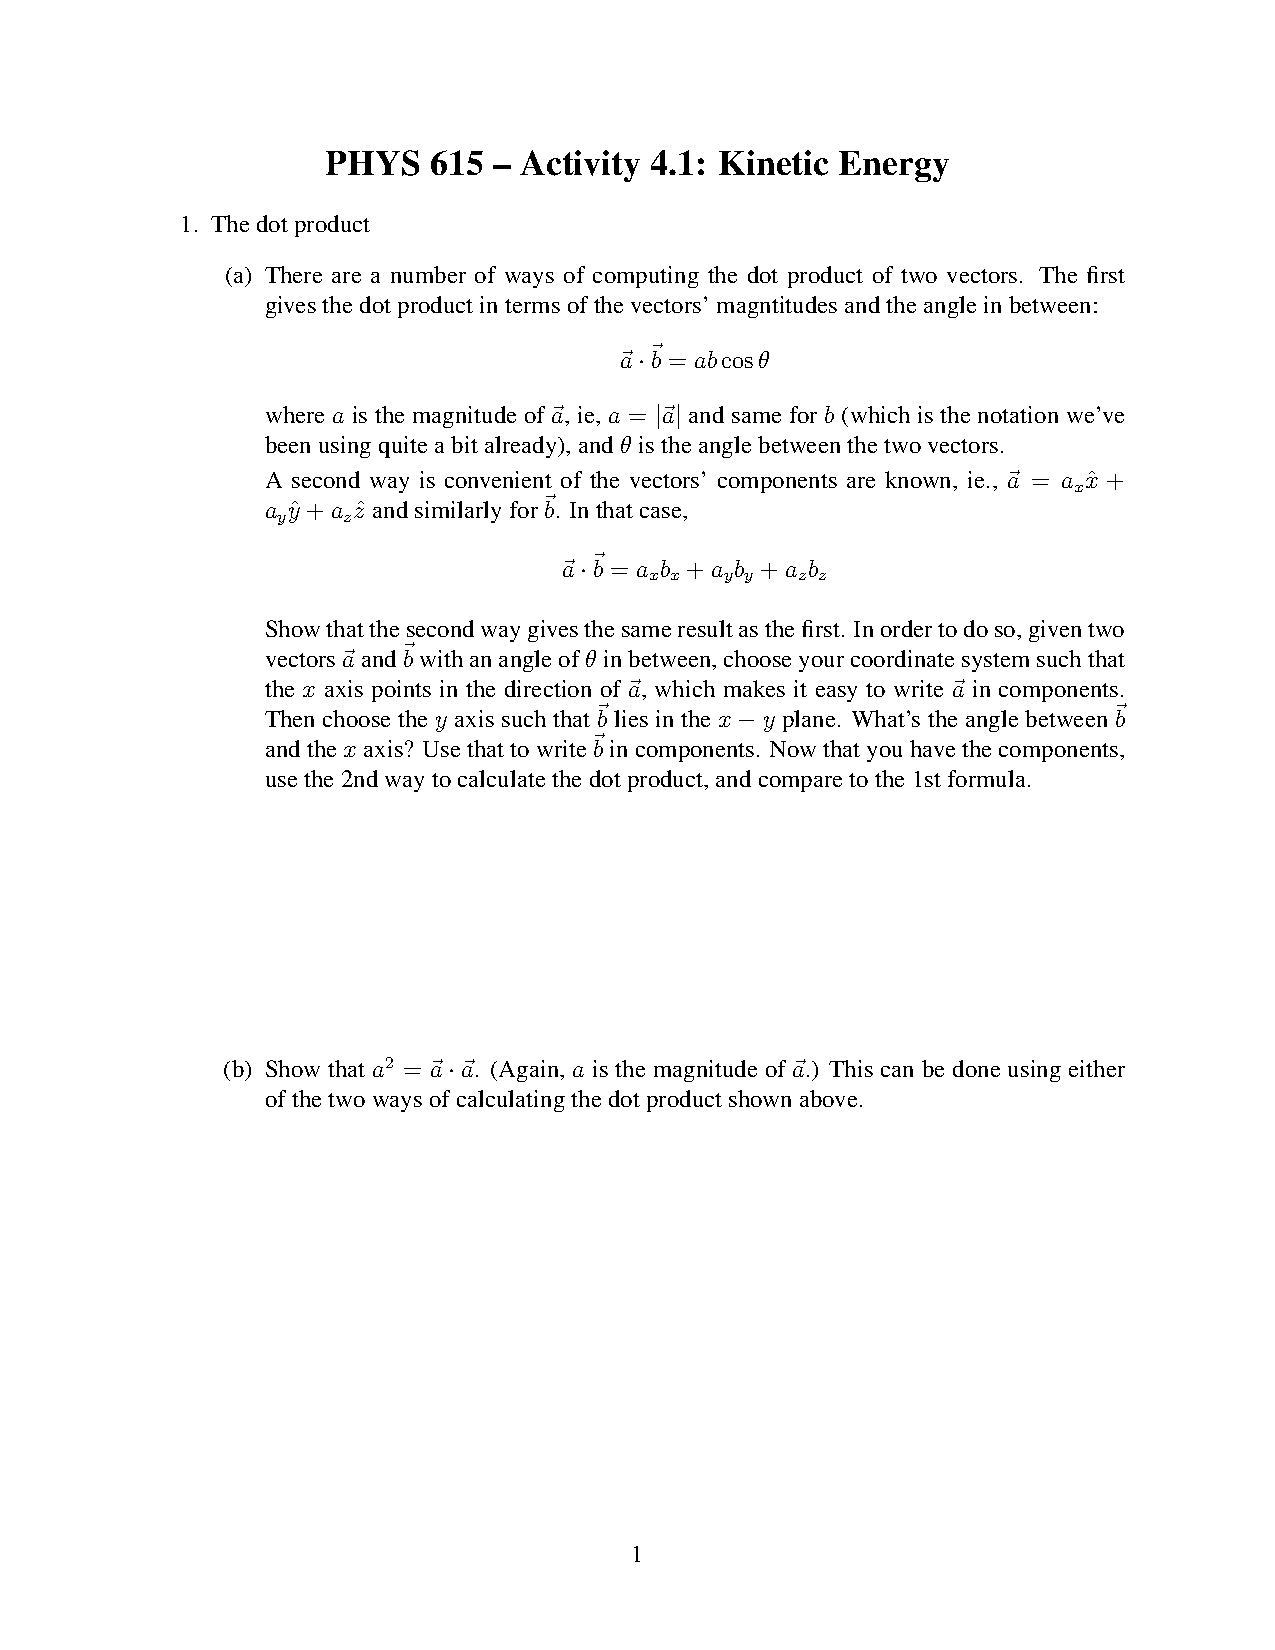
\includepdf[pages=1-]{activity4.1.pdf}
% 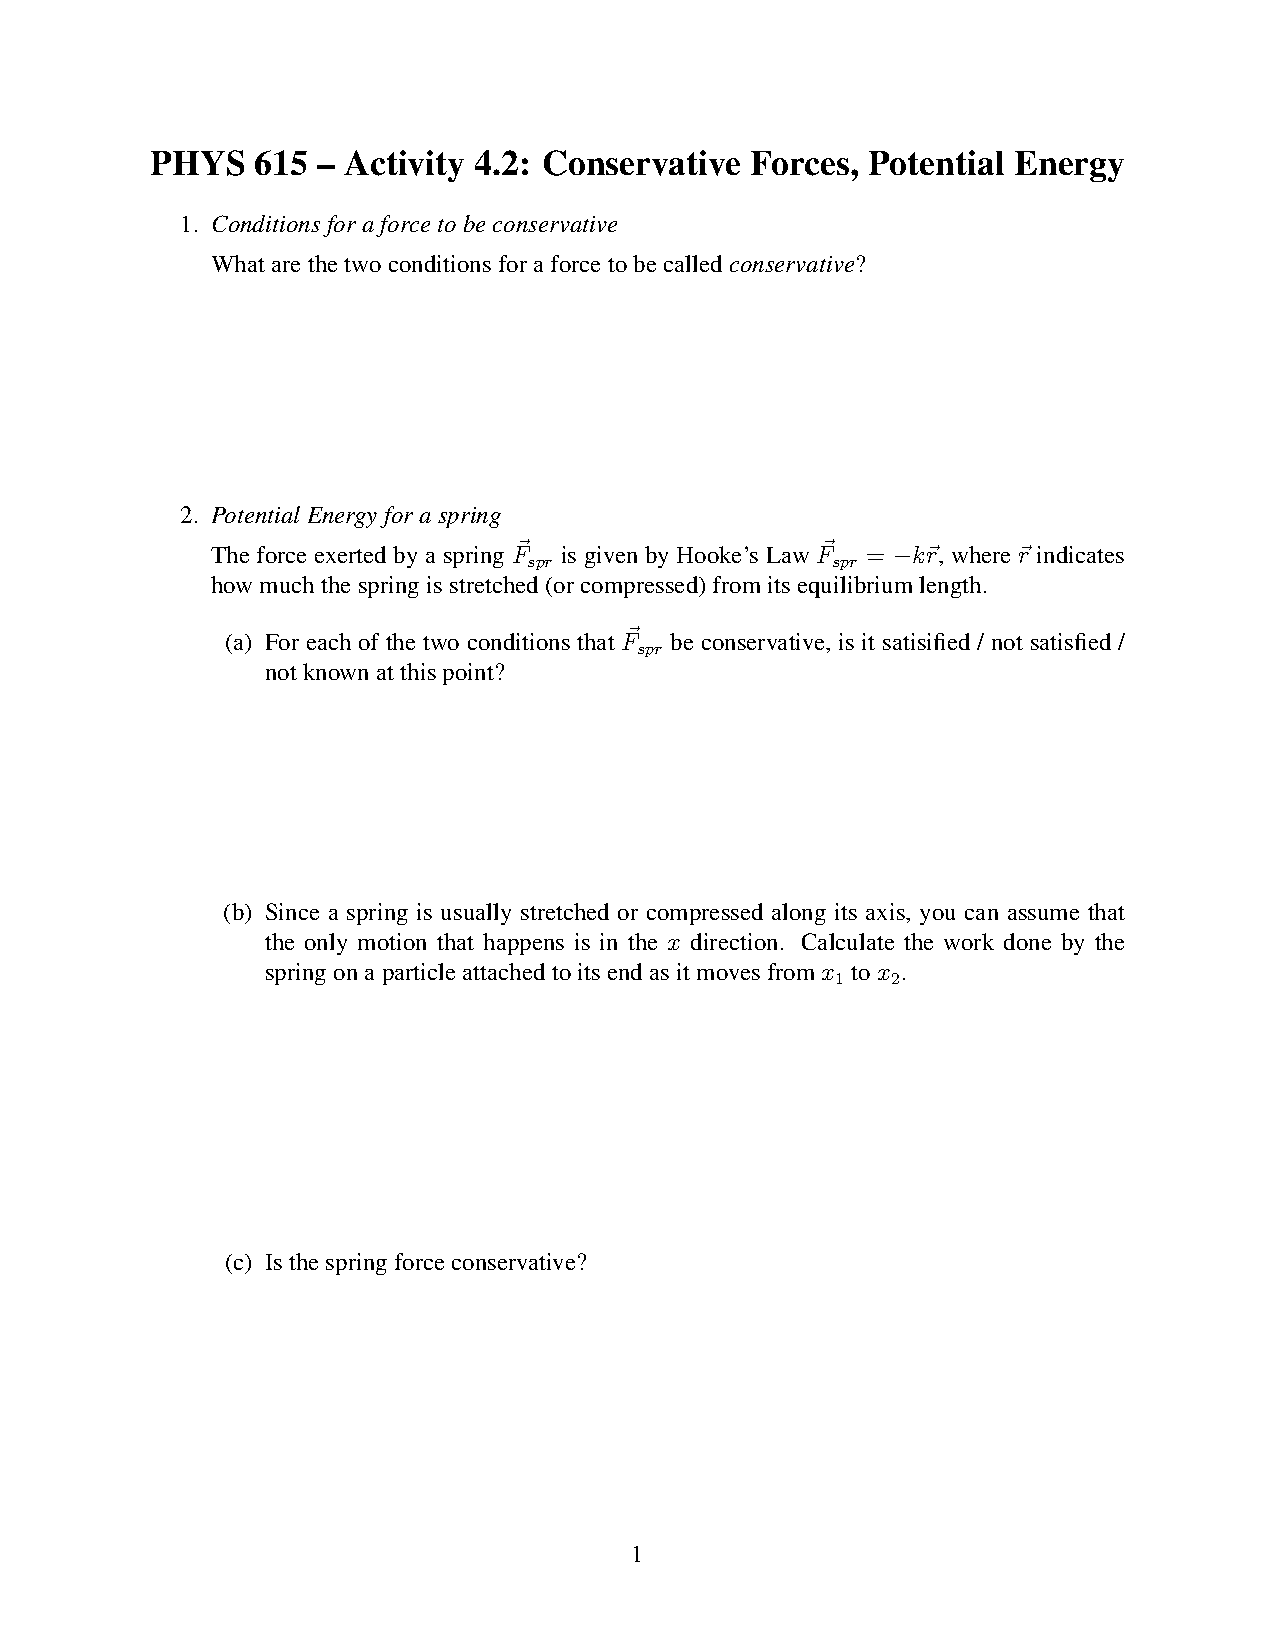
\includepdf[pages=1-]{activity4.2.pdf}
% 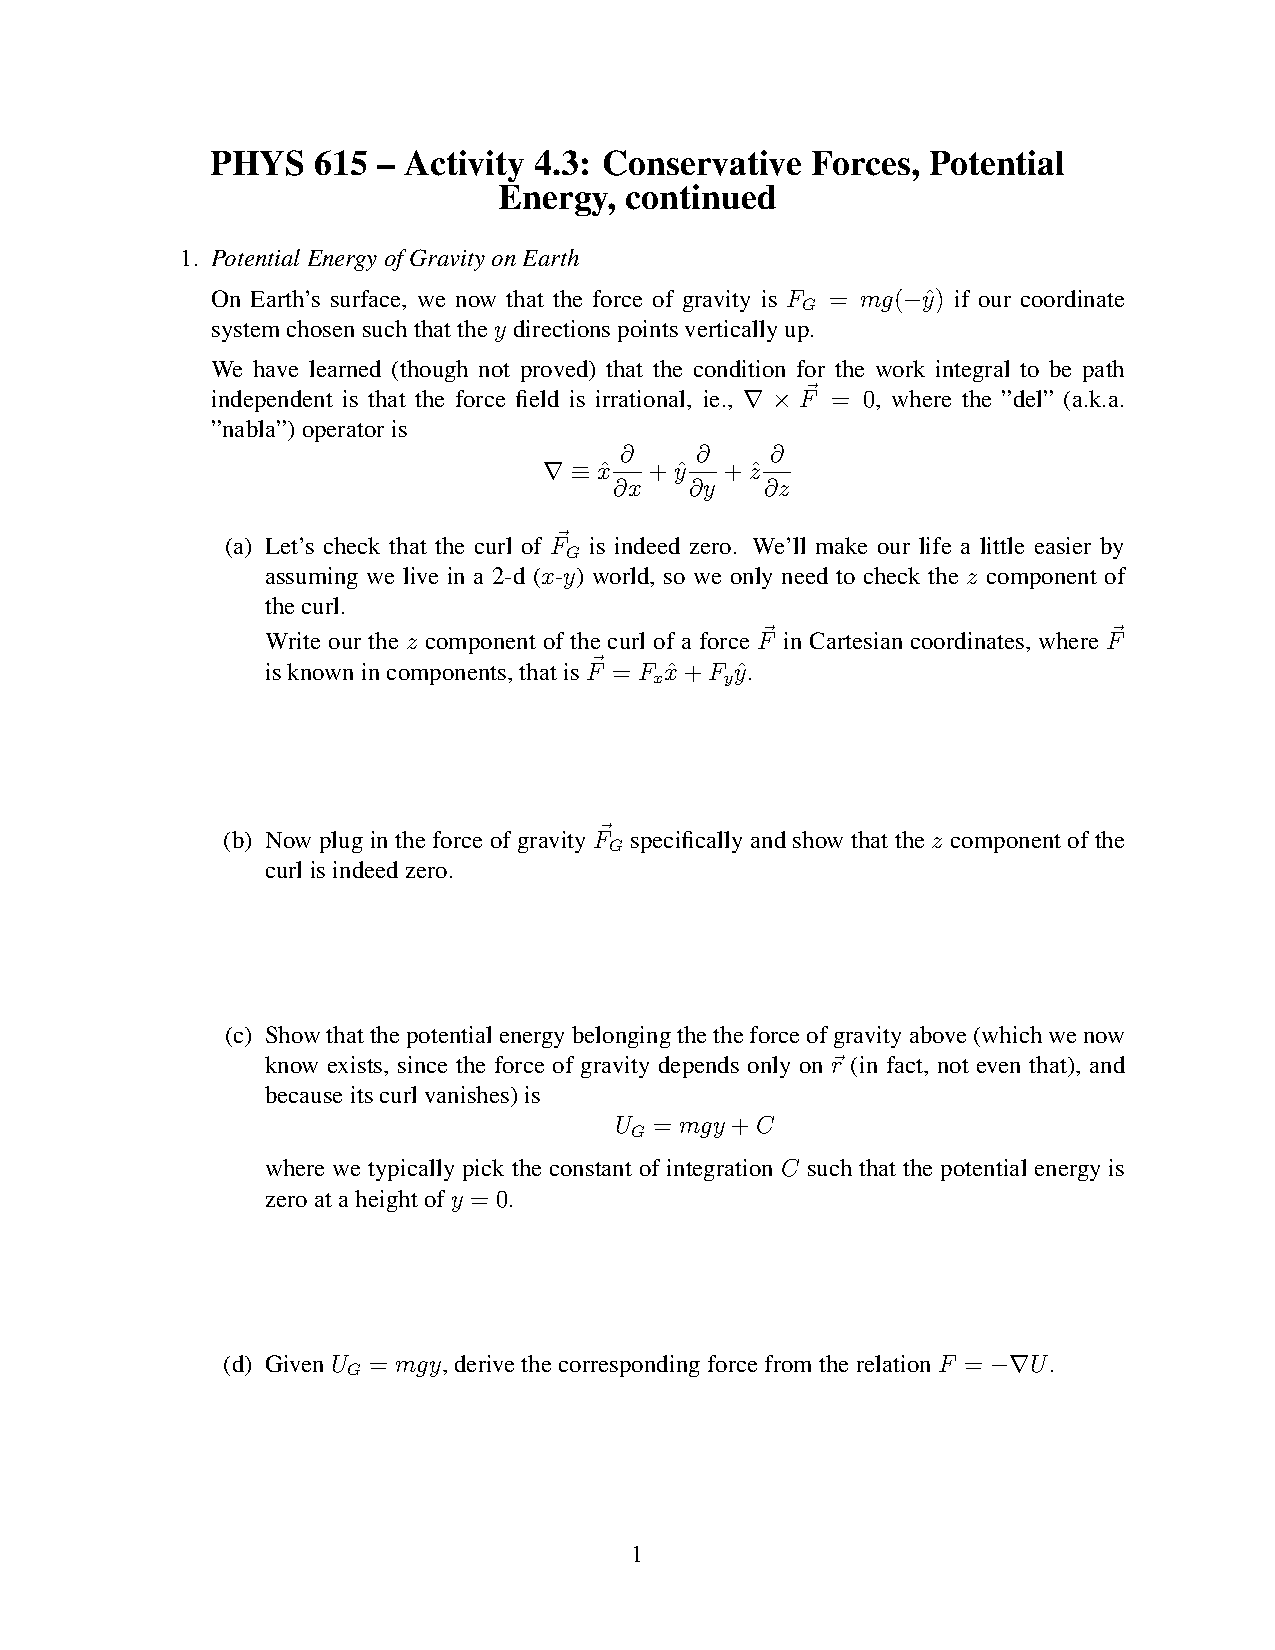
\includepdf[pages=1-]{activity4.3.pdf}

\end{document}
